\documentclass[border=10pt]{standalone}
\usepackage{tikz}\usepackage{amsmath}\usetikzlibrary{arrows.meta}
\begin{document}
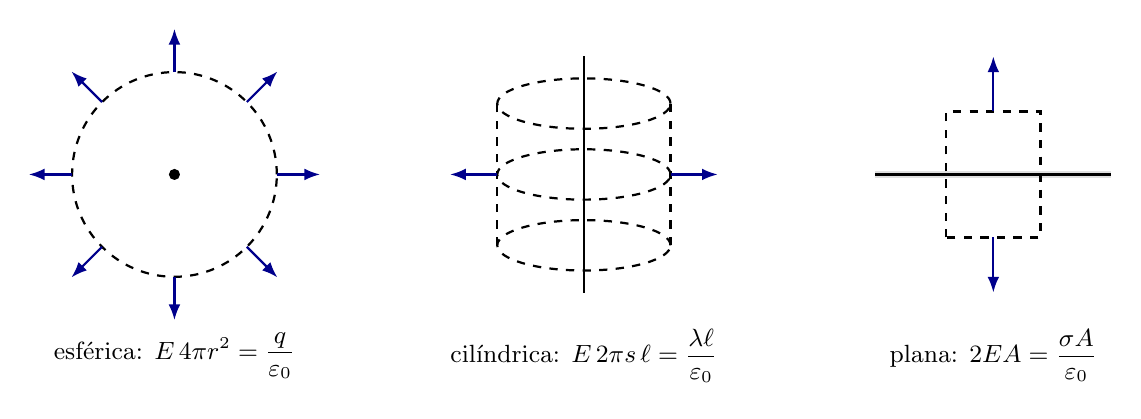
\begin{tikzpicture}[line width=0.8pt,>={Latex[length=2mm]}]
  % esfera
  \draw[dashed] (0,0) circle(1.3);
  \fill (0,0) circle(2pt);
  \foreach \a in {0,45,...,315} \draw[->,blue!55!black] (\a:1.3)--(\a:1.85);
  \node at (0,-2.3){\small esférica: $E\,4\pi r^2=\dfrac{q}{\varepsilon_0}$};
  % cilindro (linea)
  \begin{scope}[xshift=5.2cm]
    \draw[thick] (0,-1.5)--(0,1.5);
    \draw[dashed] (0,0) ellipse (1.1 and 0.32);
    \draw[dashed] (-1.1,-0.9)--(-1.1,0.9) (1.1,-0.9)--(1.1,0.9);
    \draw[dashed] (0,0.9) ellipse (1.1 and 0.32);
    \draw[dashed] (0,-0.9) ellipse (1.1 and 0.32);
    \foreach \a in {0,180} \draw[->,blue!55!black] (\a:1.1)--(\a:1.7);
    \node at (0,-2.3){\small cilíndrica: $E\,2\pi s\,\ell=\dfrac{\lambda\ell}{\varepsilon_0}$};
  \end{scope}
  % plano (pillbox)
  \begin{scope}[xshift=10.4cm]
    \fill[black!12] (-1.5,-0.05) rectangle (1.5,0.05);
    \draw (-1.5,0)--(1.5,0);
    \draw[dashed] (-0.6,-0.8) rectangle (0.6,0.8);
    \draw[->,blue!55!black] (0,0.8)--(0,1.5);
    \draw[->,blue!55!black] (0,-0.8)--(0,-1.5);
    \node at (0,-2.3){\small plana: $2EA=\dfrac{\sigma A}{\varepsilon_0}$};
  \end{scope}
\end{tikzpicture}
\end{document}
